Для верификации вычислений приложения использовались статьи написанные по реальным экспериментальным данным полученных от коллабора-ции \textit{ATLAS}. Верифиционными данными являются ограничения на эффекты $Z$-${Z}^{\prime}$ смешивания на Большом Адронном колайдере.

После открытия $Z^\prime$-бозона на БАК через процесс ДЯ, необходимо произвести некоторую диагностику связей и смешивания $Z$-$Z^\prime$, чтобы идентифицировать основную теоретическую структуру. В настоящей работе исследуются данные \textit{ATLAS} [4] и \textit{CMS} в канале дибозона.

\begin{equation} \label{eq:verify-1}
pp \rightarrow W^+W^- + X.
\end{equation}

Для поиска \textit{Z}-бозона, который возникает, например, в популярной модели с расширенным калибровочным сектором. Анализ основан на данных о столкновениях $pp$ при энергии центра масс $\sqrt{s} = 13 $ собранных группами \textit{ATLAS}~\cite{ada-wwz:2013} и \textit{CMS} на БАК. В частности, данные используются для поиска $Z$-$Z^\prime$ смешивание. На \textit{ATLAS} события $W^+W^-$ реконструируются через их полулептонные распады $W$, где один $W$-бозон распадается на заряженный лептон ($l=e,\mu$) и нейтрино, а другой на две струи, тогда как на \textit{CMS} $W$-бозон адронически распадается на две восстановленные струи. 

Процесс рождения пары $W^-W^+$-бозонов (\ref{eq:verify-1}) важен для изучения электрослабой калибровочной симметрии. Общие свойства слабых калибровочных бозонов тесно связаны с нарушением электрослабой симметрии и структуры калибровочного сектора, как и существование и структура трилинейных связей. Кроме того, канал распада дибозонов $Z^\prime$ исследует толщину калибровочной связи между новым и калибровочными бозонами стандартной модели. Кроме того, сила связи очень влияет на элементы распада и естественную ширину такого нового калибровочного бозона. Таким образом, детальное рассмотрение процесса (\ref{eq:verify-1}) с высокой точностью проверяет калибровочный сектор СM и может пролить свет на бозоны, которые могут появиться за пределами СМ. Здесь мы рассмотрим возможность наблюдения $Z^\prime$-бозона в $W^+W^-$ парного процесса на БАК, который в отличие от процесса ДЯ не является основным каналом поиска, но может помочь понять происхождение новых калибровочных бозонов.

Для верификации верхних пределов сечения распада ${Z}^{\prime} \rightarrow {W}^{+}{W}^{-} $ использована научная статья основанная на реальных экспериментальных данных~\cite{2part-pankov}. На рисунке~\ref{fig:graph-1-verify} изображены экспериментальные распределения по теориям, что полностью соответствует распределению построенного разработанным приложением (рисунок~\ref{fig:graph-1}).

\begin{figure}[!h]
	\centering
	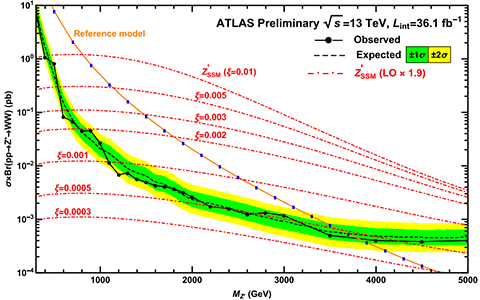
\includegraphics[width=\textwidth]{figures/graph-1-verify.png}
	\caption{Наблюдаемые и ожидаемые верхние пределы сечения распада ${Z}^{\prime} \rightarrow {W}^{+}{W}^{-} $, как функция ${Z}^{\prime}$ массы ${M}_{{Z}^{\prime}}$ полученные из обработки данных эксперимента \textit{ATLAS}~\cite{2part-pankov}}
	\label{fig:graph-1-verify}
\end{figure}

Поиски тяжелого $W^+W^-$ резонанса были выполнены на Теватроне исследовательскими группами \textit{CDF} и \textit{D0}. Группа \textit{D0} изучала резонансное рождение дибозонов до 700 ГэВ в каналах распада $lvl^\prime v^\prime$ и $lvjj$~\cite{andreev-ee:2012}. Группа \textit{CDF} также исследовала резонанс в $W^+W^-$  в канале распада $evjj$, что в результате привело к обнаружения нижних лимитов масс $Z^\prime$
и $W^\prime$-бозонов, за исключением масс превышающих 900 ГэВ, зависящих от параметра смешивания.

Исследования \textit{WW}-резонансов группами \textit{ATLAS} и \textit{CMS} с использованием, соответственно, полулептонных и адронных событий распада в $pp$ столкновениях при 13 ТэВ устанавливают массовые пределы 3 ТэВ для этих резонансов~\cite{ada-wwz:2013}. 

В этой работе изучается возможность рождения нового резонанса нейтрального спина 1 ($Z^\prime$) из доступных данных групп \textit{ATLAS} и \textit{CMS} для $W^+W^-$ распадов. В качестве результатов работы будут получены ограничения на соответствующие $Z-Z^\prime$-коэффициенты смешивания и на массу~$M_{Z^\prime}$.

Существует много теоретических моделей, которые предсказывают $Z^\prime$ с массой в диапазоне ТэВ. Мы рассмотрим модель, где $Z^\prime$ взаимодействуют со светлыми кварками и заряженными калибровочными бозонами посредством их смешивания с \textit{Z}, предполагая, что \textit{Z}-связывания имеют ту же структуру Лоренца, как и в СМ. В частности, в настоящем анализе мы сосредоточимся на калибровочном бозоне «последовательной стандартной модели» (ПСМ).

В простой модели связи \textit{Z} бозонов с фермионам (кварки, лептоны) и \textit{W}-бозонами являются прямой транскрипцией соответствующих связей стандартной модели. Заметим, что такого бозона $Z^\prime$ не ожидается в контексте калибровочных теорий, если он не имеет дополнительных связей с экзотическими фермионами. Однако он служит полезным справочным примером при сравнении ограничений из разных источников. Он также мог бы играть роль возбужденного состояния обычного \textit{Z} в моделях композитности или с дополнительными размерами в слабом масштабе.

Во многих расширенных калибровочных моделях, в то время как связи с фермионами мало чем отличаются от связей стандартной модели, $Z^\prime$ $WW$ существенно подавляется по отношению к СМ. Фактически, в расширенной калибровочной модели стандартная модель трилинейной калибровочной связи бозонов, $g_{WWZ}(=\cot \theta_{W})$ заменяется на $g_{WWZ}\rightarrow\xi \cdot g_{WWZ}$, где $\xi = C \cdot (M_{W}/M_{Z^\prime})^2$ коэффициент смешивания и $C$ - коэффициент масштабирования прочности связи [5]. Мы установим границы сечения для таких $Z^\prime_{SSM}$ как функция массы $M_{Z^\prime}$ и $\xi$. Следует отметить, что большинство результатов поиска $Z^\prime$ показывают, что массовые пределы $\xi = (M_{W}/M_{Z^\prime})^2$.

Изучение процесса рождения ${W}^{+}{W}^{-}$ бозонной пары на Большом адронном коллайдере позволяет исследовать спонтанное нарушение калибровочной симметрии стандартной модели (\textit{SM}) и может использоваться для поиска новых явлений за пределами \textit{SM}. Дополнительные нейтральные векторные ${Z}^{\prime}$-бозоны, распадающиеся на заряженные калибровочные векторные пары бозонов ${W}^{+}{W}^{-}$, предсказаны во многих сценариях новой физики, включая модели с расширенным калибровочным сектором. Процесс $pp \rightarrow {W}^{+}{W}^{-}$  позволяет установить жесткие ограничения на угол смешивания $\xi$ для $Z$-${Z}^{\prime}$ и массу ${Z}^{\prime}$, ${M}_{{Z}^{\prime}}$. В настоящей работе впервые получены ограничения на параметры ${Z}^{\prime}$ смешивания в плоскости $\xi$–${M}_{{Z}^{\prime}}$, полученные из экспериментальных данных \textit{ATLAS} и \textit{CMS} на \textit{LHC} при энергии 13 ТэВ и светимостями 36,1 и 35,9 фб${}^{−1}$, соответственно.

Многие новые физические сценарии (\textit{NP}) за пределами \textit{SM}, включая суперструнные и лево-симметричные модели, предсказывают существование новых нейтральных и заряженных калибровочных бозонов. 

Поиск этих новых нейтральных ${Z}^{\prime}$ и заряженных ${W}^{\prime}$ калибровочных бозонов является важным аспектом экспериментальной программы физики высокоэнергетических коллайдеров. 

\begin{figure}[!h]
	\centering
	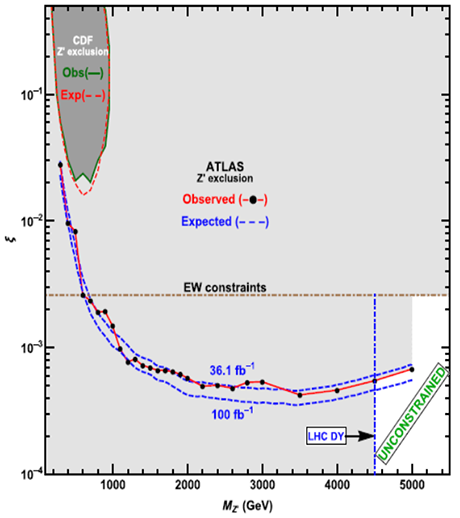
\includegraphics[width=\textwidth]{figures/verify-1.png}
	\caption{Ограничения на угол смешивания $Z$-${Z}^{\prime}$ полученные из обработки данных эксперимента \textit{ATLAS}~\cite{2part-pankov}}
	\label{fig:verify-1}
\end{figure}

Здесь рассматриваются  эффекты ${Z}^{\prime}$-бозонов. Существующие ограничения на прямое рождение на \textit{LHC} и виртуальные эффекты на Большом электронно-позитронном коллайдере (\textit{LEP}) путем интерференции или смешения с $Z$-бозоном подразумевают, что любой новый ${Z}^{\prime}$-бозон довольно тяжелый и очень мало смешивается с $Z$-бозоном. В зависимости от рассматриваемой теоретической модели массы ${Z}^{\prime}$ порядка 4,5 ТэВ и углы смешивания $Z$-${Z}^{\prime}$ на уровне нескольких промилле исключены. Угол смешивания сильно ограничен очень высокоточными экспериментами на \textit{LEP} и линейным коллайдером \textit{SLAC} (\textit{SLC}).

\begin{figure}[!h]
	\centering
	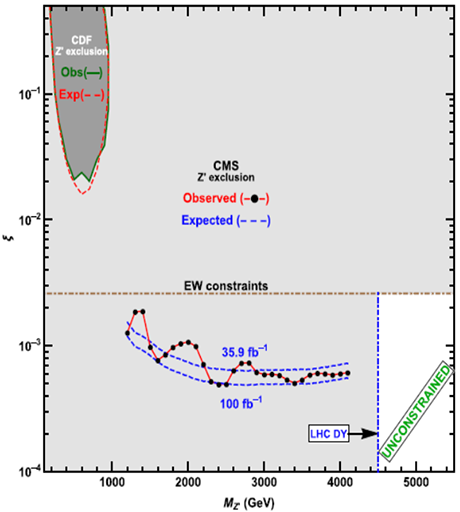
\includegraphics[width=\textwidth]{figures/verify-2.png}
	\caption{Ограничения на угол смешивания $Z$-${Z}^{\prime}$ полученные из обработки данных эксперимента \textit{CMS}~\cite{2part-pankov}}
	\label{fig:verify-2}
\end{figure}

Более подробно детали анализа данных экспериментов \textit{ATLAS} и \textit{CMS} представлены в работе~\cite{2part-pankov}. 

Основной задачей приложения является получение ограничения на угол смешивания ${Z}^{\prime}$-бозонов в протон-протонных столкновениях. На рисунке~\ref{fig:graph-result} изображены ограничения построенные по данным имитационного моделирования, которые и соответствуют полученным эксперементальным данным $\xi$ < 0,0004 (рис.~\ref{fig:verify-1}, рис.~\ref{fig:verify-2}), а так же рассчитаны ограничения для значений светимости 1000 фб${}^{−1}$ и 3000 фб${}^{−1}$, которые составили ${10}^{-4}$ и $6*{10}^{-5}$ соотвественно.


